%% The following is a directive for TeXShop to indicate the main file
%%!TEX root = diss.tex

\chapter{Introduction}
\label{chap:intro}

Listeners are faced with a large degree of phonetic variability when interacting with their fellow language users.  
Speakers differ in size, gender, and sociolect which makes speech sound categories overlap in acoustic dimensions.
Despite this variation, listeners can interpret disparate and variable productions as belonging to a single word type or sound category, a phenomenon referred to as perceptual constancy \citep{Shankweiler1977, Kuhl1979} or recognition equivalence \citep{Sumner2013}.
One of the processes for achieving this constancy is perceptual learning whereby perceivers update a perceptual category based on contextual factors.
While perceptual learning is a response to speaker variability, there is also variability on the part of the listener.
They may be distracted by concurrent demands or they may be focused on different aspects of the speech.
If the speaker has a peculiar trait, a listener may be overly focused on that trait, to the detriment of overall understanding.
Perceptual learning is typically framed in terms of speaker variation.
In contrast, this dissertation examines the effect of listener variability on perceptual learning.

In the speech perception literature perceptual learning has two distinct, yet related usages.
The first refers to learning to understand a group of speakers that share a common characteristic, such as a nonnative accent \citep{Bradlow2008}.
The second refers to the updating of specific distributions of a single speaker's sound category following exposure \citep{Norris2003}.
In this dissertation, the usage of perceptual learning is the latter.

The primary locus of investigation within the perceptual learning literature is generalization to novel contexts.
In most studies, exposure to modified sound categories generalizes to other words and nonwords when the modified exposure tokens are embedded in real words \citep{Norris2003, Reinisch2013}.  
This paradigm is referred to as lexically-guided perceptual learning, as listeners are exposed to the modified sounds in the context of real words in a lexical decision task.
On the other hand, generalization appears to be more limited when perceptual learning is induced through visually-guided paradigms in which listeners are exposed to a modified category through matching it to an unambiguous video signal.  
The perceptual learning exhibited from these visually-guided experiments is only found to influence the specific nonword that perceivers are exposed to and not other similar nonwords \citep{Reinisch2014}.  
This kind of exposure-specificity effect has been widely reported in perceptual learning studies in the psychophysics literature \citep[for review]{Gibson1953}.

Why, then, does lexically-guided perceptual learning produce such generalization?
Here I posit that these results can be understood by considering the attentional set exploited in the exposure phase.
An attentional set is a strategy that is employed by perceivers to prioritize certain aspects of stimuli.
Attentional sets can be induced through instructions or through properties of stimuli themselves.
A common example in the visual domain is the attentional sets employed in visual search tasks.
If a perceiver has to find a target shape in a field of shapes, there are two possible attentional sets \citep{Bacon1994}.
The first is a singleton-detection attentional set --  a diffuse set where any salient information along any dimension will be given priority.
If the target shape is a circle in a field of squares, then the singleton-detection attentional set is elicited, because the shape to find is always a highly salient element.
Singleton detection can result in slowed reaction times if a distractor singleton (i.e. a red square) is present.
The second attentional set is the feature-detection set -- a focused set limited to the target's defining feature.
If there are multiple, redundant targets or many distractor singletons, then the singleton-detection attentional set will not be an effective strategy and feature detection will be employed.
Using feature detection, participants are not distracted by singletons.
\citet{Bacon1994} speculate that singleton detection requires less effort than feature search.
Even if participants are given instructions targeting a relevant feature, they will default to singleton detection unless it is made ineffective through stimulus design.

In the speech perception literature, two broad attentional sets have been posited \citep{Cutler1987, Pitt2012}.  
The first is a \emph{comprehension-oriented} or \emph{diffuse} attentional set -- this is the attentional set assumed to operate during normal language use.  
When oriented towards comprehension, listeners are focused on comprehending the intended message of the speech, and a comprehension set is promoted by tasks that focus on word identity and word recognition.
The comprehension-oriented attentional set is elicited in lexically-guided perceptual learning paradigms through their use of lexical decision tasks and the embedding of modified sound categories in word tokens. 
A second kind of attentional set is a \emph{perception-oriented} or \emph{focused} attentional set, where a listener is focused more on the low-level signal properties of the speech rather than the message.
The perception-oriented attentional set is promoted by tasks such as phoneme/syllable monitoring or mispronunciation detection.
The tasks used in visually-guided perceptual learning and perceptual learning within the psychophysics literature can be thought of as eliciting this attentional set, due to their focus on stimuli that are devoid of linguistic meaning.

Comprehension and perception are, of course, interconnected concepts. 
For the purposes of this thesis, I largely follow the distinction drawn in \citet{Pitt2012}. 
Comprehension is the perception of the speaker's intended meaning.
In other words, it is the perception of \emph{linguistic objects} and not necessarily that of the signal.
Perception is defined as the perception of the speech as pronounced.
Perception, then, is for the fine detail of the signal (e.g., a specific spectral shape for a sibilant fricative). 
In terms of theories of speech perception, comprehension targets more the abstract linguistic representations (sound categories, words, etc.), and perception targets more the fine-detailed episodic traces of those abstract representations.
Attention to linguistic properties (i.e. syntactic category) or signal properties (i.e. talker gender) has been shown to change the relative strengths of encoding for abstract or episodic representations \citep{Goldinger1996,Theodore2015}.
These differences in attention correspond well to the attentional sets proposed above for comprehension and perception.

The core hypothesis of this dissertation is that perceivers who adopt a more comprehension-oriented attentional set will show more generalization than those who adopt a more perception-oriented attentional set.
To test this hypothesis, I use a lexically-guided perceptual learning paradigm to expose listeners to an /s/ category modified to sound more like /\textesh/.  
Groups of participants differ in whether comprehension-oriented or perception-oriented attentional sets are favored when processing the modified /s/ category based on experimental manipulations.
The favoring of attentional sets are implemented in four ways across the three experiments presented in this dissertation.  
Two manipulations are linguistic in nature, one is instruction-based, and the fourth is stimulus-based.
The rest of this section is devoted to an overview of these manipulations and their motivations.

Before introducing the manipulations themselves, a definition of perceptual salience is necessary.
Salience is a widely-used and poorly-defined term across the literature.
For the purposes of this dissertation I adopt the following definition:  an element is salient if it is unpredictable from context and/or easily distinguishable from other possible elements.  
The sound category that is being learned in this dissertation already has salient signal properties (e.g., in the form of high frequency, relatively high amplitude, aperiodic noise).
Increasing the perceptual salience of the modified /s/ category is a function of embedding it a linguistic position with little conditioning context or increasing the acoustic distance from a typical /s/ production.

I argue that increased perceptual salience promotes a more perception-oriented attentional set.
In general, psycholinguistic studies have a small number of target trials and a large number of unrelated filler trials.
By doing so, it is argued that participants will be less likely to become aware of the true purpose of the experiment until debriefing.
Changing the nature of the filler trials can induce attentional set changes: if more fillers are words rather than nonwords, a comprehension-oriented attentional set is promoted \citep{Mirman2008}.
Increasing the number of target trials can also induce attentional set changes.
Instructing participants to attend to a modified sound in the stimuli has less of an effect when there are proportionally more of those trials \citep{Pitt2012}.
Put another way, if the modified sounds are salient due to prevalence, participants are more likely to notice the targets and adopt a more perception-oriented attentional set without explicit instructions.
Increasing perceptual salience through stimulus design in this dissertation is predicted to have the same effect.

The first linguistic manipulation used to promote different attentional sets is the position of the modified /s/ in the exposure words.  
Accurate perception is most critical when expectations are low, as perception of highly expected elements serves a more confirmatory role \citep{Marslen-Wilson1978, Gow1995}.
Some groups of participants are exposed to the modified sound only at the beginnings of words (e.g. \emph{silver}, \emph{settlement}) and other groups are exposed to the category only in the middle of words (e.g. \emph{carousel}, \emph{fossil}).
Word-initial positions lack the expectations afforded to the word-medial positions, and lexical information exhibits less of an effect on word-initial positions as compared to later positions \citep{Pitt2006}.
As such, word-initial exposure is predicted to increase the perceptual salience of the modified /s/ category and promote a more perception-oriented attentional set.
In contrast, word-medial exposure is predicted to promote a more comprehension-oriented attentional set.
Experiments 1 and 2 use this manipulation in Chapter~\ref{chap:lexdec}, and further background is given in Section~\ref{sec:lexicalbias} of this chapter.

The second linguistic manipulation employed is the context in which a word appears.  
In Experiments 1 and 2, participants are exposed to the modified sound category in words in isolation, as in previous work \citep{Norris2003}.  
However, in Experiment 3, the words containing the sound category have been embedded in sentences that are either predictive or unpredictive of the target word.
Use of sentence frames is predicted to promote comprehension-oriented attentional sets more than words in isolation.
Increasing the predictability of a word increases the expectations for the sounds in those words as well, mirroring the word-position manipulation above.
Further background on the use of the sentence frames is given in Section~\ref{sec:semanticpredictability}.

Participants in all three experiments receive the same general instructions for the exposure task, but one group of participants in each experiment receive additional instructions about the nature of the /s/ category, following previous studies \citep{Pitt2012}.
Without any additional instructions, the task is predicted to promote a comprehension-oriented attentional set.
The instructions about /s/ are expected to promote a perception-oriented attentional set.
Section~\ref{sec:attention} contains background on attention and instructions.

The stimulus-based manipulation is the degree of typicality of the modified /s/ category -- Experiments 1 and 2 differ in this respect. 
In line with previous work \citep{Norris2003}, participants in Experiment 1 are exposed to a modified category halfway between /s/ and /\textesh/. 
Participants in Experiment 2 are exposed to an even more atypical /s/ -- the modified fricative is more /\textesh/-like than /s/-like.  
Exposure to an atypical category is predicted to promote a more perception-oriented attentional set because its atypicality is predicted to be more perceptually salient.

The structure of the thesis is as follows.
This chapter provides an overview of relevant literature on perceptual learning (Section~\ref{sec:perceptuallearning}), linguistic expectations (Section~\ref{sec:linguistic}), attention (Section~\ref{sec:attention}), and category typicality (Section~\ref{sec:signal}) as they relate to and motivate the three experiments of this dissertation.
Chapter~\ref{chap:lexdec} details two experiments using a lexically-guided perceptual learning paradigm, each with different conditions for levels of lexical bias and attention.  
The two experiments differ in the acoustic properties of the exposure tokens, with the first experiment using a slightly atypical /s/ category that is halfway between /s/ and /\textesh/.
The second experiment using a more atypical /s/ category that is more /\textesh/-like than /s/-like.  
Chapter~\ref{chap:sent} details an experiment using a novel exposure paradigm that manipulates semantic predictability to increase the linguistic expectations during exposure.
Finally, Chapter~\ref{chap:conclusion} summarizes the results and places them within the larger literature.
The perceptual learning literature has generally used consistent processing conditions to elicit perceptual learning effects, and a goal of this dissertation is to examine the robustness and degree of perceptual learning across conditions that promote more comprehension- or more perception-oriented attentional sets.

\section{Perceptual learning}
\label{sec:perceptuallearning}

Perceptual learning is a well established phenomenon in the psychophysics literature. 
Training can improve a perceiver's ability to discriminate in many disparate modalities (e.g., visual acuity, somatosensory spatial resolution, weight estimation, and discrimination of hue and acoustic pitch \citep[see][for review]{Gibson1953}). 
In the psychophysics literature, perceptual learning is an improvement in a perceiver's ability to judge the physical characteristics of objects in the world through training that assumes attention on the task, but does not require reinforcement, correction, or reward.
This definition of perceptual learning corresponds more to what is termed ``selective adaptation'' in the speech perception literature rather than what is termed ``perceptual learning'', ``perceptual adaptation'' or ``perceptual recalibration.''  
In speech perception, selective adaptation is the phenomenon where listeners that are exposed repeatedly to a narrow distribution of a sound category narrow their own perceptual category.
This results in a change in variance of the category, but not of the mean of the category along some acoustic-phonetic dimension \citep{Eimas1973,Samuel1986,Vroomen2007}.
Perceptual learning or recalibration in the speech perception literature is a more broad updating of perceptual categories resulting in changed means and/or variance \citep{Norris2003, Vroomen2007}.

\citet{Norris2003} began the recent set of investigations into lexically-guided perceptual learning in speech.
Norris and colleagues exposed one group of Dutch listeners to a fricative halfway between /s/ and /f/ at the ends of words like \emph{olif} ``olive'' and \emph{radijs} ``radish'', while exposing another group to the ambiguous fricative at the ends of nonwords, like \emph{blif} and \emph{blis}.
Following exposure, both groups of listeners were tested on their categorization of a fricative continuum from 100\% /s/ to 100\% /f/. 
Listeners exposed to the ambiguous fricative at the end of words shifted their categorization behavior, while those exposed to the same sounds at the end of nonwords did not.  The exposure using words was further differentiated by the bias introduced by the words.  That is, half the tokens ending in the ambiguous fricative formed a word if the fricative was interpreted as /s/ but not if it was interpreted as /f/, and the others were the reverse.  
Listeners exposed only to the /s/-biased tokens categorized more of the /f/-/s/ continuum as /s/, and listeners exposed to /f/-biased tokens categorized more of the continuum as /f/.  
The ambiguous fricative was associated with either /s/ or /f/ according to the bias induced by the word, which led to an expanded category for that fricative at the expense of the other category.
These results crucially show that perceptual categories in speech are malleable, and that the linguistic system of the listener facilitates generalization to that category in new forms and contexts.

In addition to lexically-guided perceptual learning, unambiguous visual cues to sound identity can cause perceptual learning as well; this is referred to as perceptual recalibration.
In \citet{Bertelson2003}, an auditory continuum from /aba/ to /ada/ was synthesized and paired with a video of a speaker producing /aba/ or /ada/.  
Participants first completed a pretest that identified the maximally ambiguous step of the /aba/-/ada/ auditory continuum. 
In eight blocks, participants were randomly exposed to the ambiguous auditory token paired with video for /aba/ or /ada/.  Following each block, they completed a short categorization test.  
Participants showed perceptual learning effects, such that they were more likely to respond with /aba/ if they had been exposed to the video of /aba/ paired with the ambiguous token in the preceding block, and vice versa for /ada/.

%\citet{vanLinden2007} compared the perceptual recalibration effects from the visually-guided perceptual learning paradigm \citep{Bertelson2003} to the more lexically-guided perceptual learning paradigm.
%Perceptual learning effects from visually- and lexically-guided paradigms had comparable sizes, lasted equally as long, were enhanced when presented with a contrasting sound, and were both unaffected by periods of silence between exposure and categorization.
%However, the lexically-guided paradigm in \citet{vanLinden2007} differs from the normal lexical decision paradigm used in most lexically-guided perceptual learning experiments \citep{Norris2003}.
%Participants in the lexically-guided paradigm did not perform a lexical decisions, but rather just listened to words containing an ambiguous category.
%No fillers were present during lexical exposure and participants completed categorization tasks at the beginning of the experiment and interspersed with exposure.

Visually-guided perceptual learning in speech perception has been modeled using a Bayesian belief updating framework \citep{Kleinschmidt2011}.  
In their framework, the model categorizes the incoming stimuli based on an acoustic-phonetic feature and a binary visual feature, and then updates the distribution to reflect that categorization.
This updated conditional distribution is then used for future categorizations in an iterative process.  
\citet{Kleinschmidt2011} effectively model the results of the behavioral study in \citet{Vroomen2007} in a Bayesian framework, with models fit to each participant capturing the perceptual recalibration and selective adaptation shown over the course of the experiment.
The Bayesian belief updating framework is largely specific to the visually-guided perceptual learning paradigm.

A similar, but more general Bayesian framework for perception and action in cognition is the predictive coding model \citep{Clark2013}, schematized in Figure~\ref{fig:predictivecoding}.
This framework uses a hierarchical generative model that aims to minimize prediction error between bottom-up sensory inputs and top-down expectations.  
Mismatches between the top-down expectations and the bottom-up signals generate error signals that are used to modify future expectations.  
Perceptual learning then is the result of modifying expectations to match learned input and reduce future error signals.
The lowest levels of the hierarchical model have the most detailed representations.
Representations lose detail and become more abstract the higher in the hierarchy they are.
Models of speech perception generally propose representations that encode both abstract and episodic information \citep[e.g.][]{McLennan2003}.
Abstract and episodic information would map to higher and lower levels of representation in the predictive coding framework, respectively.

\begin{figure*}[!ht]
\caption{Schema of the predictive coding framework \citep{Clark2013}.  Nodes are sensory representations that become more abstract the higher they are in the hierarchy. Blue arrows represent expectations, red arrows are error signals, and yellow is the actual sensory input.}
\label{fig:predictivecoding}
\begin{center}
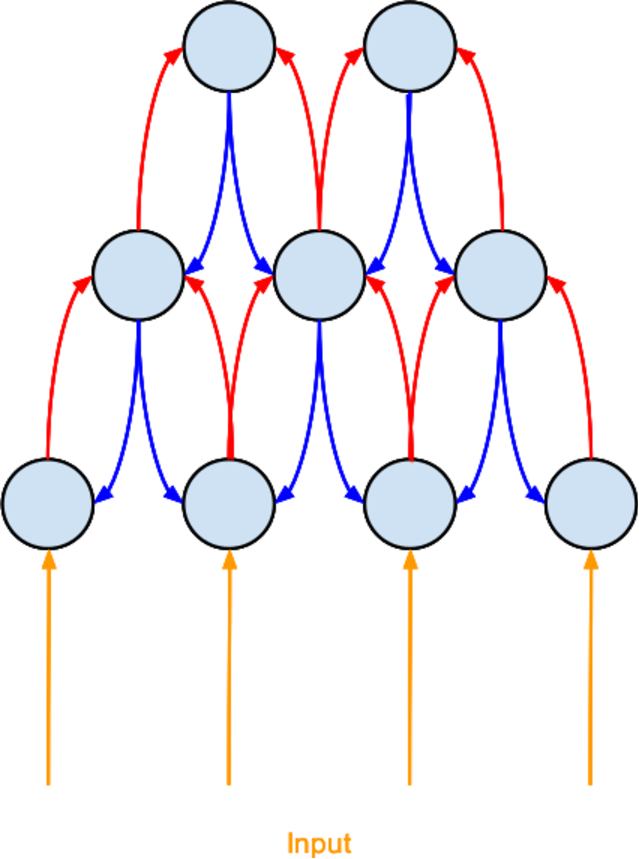
\includegraphics[width=0.5\textwidth]{pictures/predictive_coding}
\end{center}
\end{figure*}

Perceptual learning in the psychophysics literature has shown a large degree of exposure-specificity, where observers show learning effects only on the same or very similar stimuli as those they were trained on. 
As such, perceptual learning has been argued to reside in or affect the early sensory pathways, where stimuli are represented with the greatest detail \citep{Gilbert2001}.  
Visually-guided perceptual learning has also shown a large degree of exposure-specificity, where participants do not generalize cues across speech sounds \citep{Reinisch2014} or across speakers unless the sounds are sufficiently similar across exposure and testing \citep{Eisner2005, Kraljic2005, Kraljic2007, Reinisch2013a}.  
Crucially, lexically-guided perceptual learning in speech has shown a greater degree of generalization than would be expected from a purely psychophysical standpoint.  
The testing stimuli are in many ways quite different from the exposure stimuli, with participants trained on multisyllabic words ending in an ambiguous sound and tested on monosyllabic words \citep{Reinisch2013} and nonwords \citep{Norris2003, Kraljic2005}, though exposure-specificity has been found when exposure and testing use different positional allophones \citep{Mitterer2013}.

Why is lexically-guided perceptual learning more context-general?
The experiments performed in this dissertation provide evidence that this context-generality is the result of a listener's attentional set, which can be influenced by linguistic, instruction and stimulus properties.
A comprehension-oriented attentional set, where a listener's goal is to understand the meaning of speech, promotes generalization and leads to greater perceptual learning.  
A purely perception-oriented attentional set, where a listener's goal is to perceive specific qualities of a signal, does not promote generalization.
The experiments in this dissertation use the lexically-guided perceptual learning paradigm, which uses tasks oriented towards comprehension, so generalization is to be expected in general, but the more perception-oriented the attentional set, the less perceptual learning should be observed.
In terms of a Bayesian framework with error propagation, a more perception-oriented attentional set may keep error propagation more local, resulting in the exposure-specificity seen more in the psychophysics literature.
A more comprehension-oriented attentional set would propagate errors farther upward in the hierarchy of expectations.
In both cases, errors would propagate to where attention is focused, but larger updating associated with farther error propagation would lead to larger observed perceptual learning effects.
These attentional sets will be explored in more detail in Section~\ref{sec:attention} following an examination of the linguistic factors that will be manipulated in the experiments in Chapters~\ref{chap:lexdec} and \ref{chap:sent}.

\section{Linguistic expectations and perceptual learning}
\label{sec:linguistic}

The linguistic manipulations used to induce different attentional sets are lexical bias and semantic predictability.
Chapter~\ref{chap:lexdec} presents two experiments using a standard lexically-guided perceptual learning paradigm, which uses lexical bias as the means to link an ambiguous sound to an unambiguous category.
In Chapter~\ref{chap:sent}, a novel, sententially-guided perceptual learning paradigm is used to further promote use of comprehension-oriented attentional sets.

\subsection{Lexical bias}
\label{sec:lexicalbias}

Lexical bias is the primary way through which perceptual learning is induced in the experimental speech perception literature.
Lexical bias, also known as the Ganong Effect, refers to the tendency for listeners to interpret a speaker's (noncanonical) production as a meaningful word rather than a nonsense word.  
For instance, given a continuum from a nonword like \emph{dask} to a word like \emph{task} that differs only in the initial sound, listeners are more likely to interpret any step along the continuum as the word endpoint rather than the nonword endpoint compared to a continuum where neither endpoint is a word \citep{Ganong1980}. 
This bias is exploited in perceptual learning studies to allow for noncanonical, ambiguous productions of a sound to be readily linked to pre-existing sound categories.
In terms of the attentional sets proposed in this dissertation, lexical effects, including lexical bias, arise due to comprehension-oriented attentional sets.

Comprehension-oriented attentional sets are not limited to comprehension tasks.
Lexical effects have also been found for reaction time in phoneme detection tasks:
sounds are detected faster in words than in nonwords.
However, such lexical effects are dependent on the attentional set being employed.  
If the stimuli are sufficiently repetitive (e.g. all having the same CV shape) the lexical bias effects disappear \citep{Cutler1987}.
The monotony or variation of filler items is sufficient to bias listeners towards perception-oriented or comprehension-oriented attentional sets, respectively.
The lexical status of the filler items contributes to attentional set adoption as well.
Lexical effects are found when the proportion of word fillers is high, but disappear when the proportion of nonword fillers is high \citep{Mirman2008}.

%Word length
The lexical effect of interest in this dissertation is lexical bias.
The degree to which a word biases the perception of a sound is primarily determined by properties of the word.
Longer words show stronger lexical bias than shorter words \citep{Pitt2006}.  
Continua formed using trisyllabic words, such as \emph{establish} and \emph{malpractice}, were found to show consistently larger lexical bias effects than monosyllabic words, such as \emph{kiss} and \emph{fish}.  
\citet{Pitt2006} also found that lexical bias from trisyllabic words was robust across experimental conditions (e.g., compressing the durations by up to 30\%), but lexical bias from monosyllabic words was more fragile and condition dependent.
The lexical bias effects shown by monosyllabic words only approached those of trisyllabic words when the participants were told to keep response times within a certain margin and given feedback when the response time fell outside the desired range.
The reaction time monitoring could have added a greater cognitive load for participants, which has been shown to increase lexical bias effects \citep{Mattys2011}.
\citet{Pitt2006} argue that longer words exert stronger lexical bias due to both more conditioning information present in longer words and the greater lexical competition for shorter words.

%Position in the word
Within a given word, different positions have stronger or weaker lexical bias effects.
\citet{Pitt2012} used a lexical decision task with a continuum of fricatives from /s/ to /\textesh/ embedded in words that differed in the position of the sibilant.  
They found that ambiguous fricatives later in the word, such as \emph{establish} or \emph{embarrass}, show greater lexical bias effects than the same ambiguous fricatives embedded earlier in the word, such as \emph{serenade} or \emph{chandelier}.
\citet{Pitt1993} found that for monosyllabic words, token-final targets produce more robust lexical bias effects than token-initial targets.
Lexical bias is strengthened over the course of the word.
As a listener hears more evidence for a particular word, their expectations for hearing the rest of that word increase.

%Samuel1981
One final research paradigm that has investigated lexical biases is phoneme restoration tasks \citep{Samuel1981}.  
In this paradigm, listeners hear words with noise added to or replacing sounds and are asked to identify whether noise completely replaced part of the speech or noise was simply added to the speech.  
Lower sensitivity to noise addition versus noise replacement and increased bias for responding that noise has been added is indicative of phoneme restoration -- that is, listeners are perceiving sounds not physically present in the signal.  
\citet{Samuel1981} identified several factors that increase the likelihood of the phoneme restoration effect.
In the lexical domain, words are more likely than nonwords to have phoneme restorations.  
More frequent words are also more likely to exhibit phoneme restoration effects, and longer words also show greater phoneme restoration effects.  
Position of the sound in the word also influences listeners' decisions, with non-initial positions showing greater effects. 
The other influences on phoneme restoration discussed in \citet{Samuel1981}, namely the signal properties and sentential context are discussed in subsequent sections.

Lexical bias effects are found across a wide range of tasks involving speech.
However, lexical bias effects are not uniform across the word.
Various models of lexical access give a large role to the initial sounds in the word \citep{Marslen-Wilson1978, Gow1995}.
In such models, initial perception of sounds plays a disproportionate role in providing lexical identity, allowing later sounds to be perceived in reference to the initially perceived lexical identity.
In spontaneous speech, sounds are more likely to be produced canonically in early positions than in later positions \citep{Pitt2012}.
In terms of the predictive coding framework \citep{Clark2013}, decreased lexical bias would result from the lack of (or decreased) expectations from higher levels of representation.

Lexical effects are generally argued to be the result of attentional sets rather than cause \citep{Cutler1987, Pitt2012}.
I propose that ambiguous sounds that are salient, in this case due to their position in the word, cause listeners to adopt a more perception-oriented attentional set over the course of the experiment.
Under this proposal, increasing the perceptual salience of a few ambiguous sounds is functionally equivalent to having many ambiguous sounds that are not as salient.
That is, having 20 modified /s/ tokens at the beginnings of words is similar to having 40 modified /s/ tokens at the ends of words (with the same overall number of trials) or to 20 modified /s/ tokens that are less typical of /s/.
In both cases, the likelihood of the participant exogenously noticing the ambiguous sound is higher, and so too is their likelihood of adopting that into their strategy for completing the task.
The experiments in this dissertation do not fully test this proposal, as the number of exposure tokens is never manipulated.
However, it does predict that less typical modified sounds (discussed in Section~\ref{sec:signal}) embedded later in words should produce comparable perceptual learning effects as more typical modified sounds at the beginnings of words.
It is important to note that perceptual learning is predicted to occur regardless of exposure location, following previous research \citep{Norris2003,Kraljic2005, Kraljic2008, Kraljic2008,Clare2014}, but the degree of perceptual learning is predicted to be less when exposure is at the beginnings of words.
Table~\ref{tbl:predictions} lists the predicted perceptual learning effects for the linguistic manipulations and instruction.
Experiments 1 and 2  in Chapter~\ref{chap:lexdec} test the predictions related to lexical bias.

\begin{table}[ht]
\caption{Summary of predictions for size of perceptual learning effects under different linguistic expectations and attention.}
\label{tbl:predictions}
\centering
\small
\begin{tabular}{cccccc}
\toprule
                  &                   & \multicolumn{2}{c}{Lexical bias} & \multicolumn{2}{c}{Semantic predictability} \\
\cmidrule(r){3-4}
\cmidrule(r){5-6}
                  &                   & Word-initial    & Word-medial    & Unpredictable        & Predictable          \\
\midrule
\multicolumn{2}{c}{Regular attention} & Smaller effect  & Larger effect  & Larger effect       & Largest effect        \\
\multicolumn{2}{c}{Attention to /s/}  & Smaller effect  & Smaller effect & Smaller effect       & Smaller effect  \\
\bottomrule    
\end{tabular}
\end{table}

\subsection{Semantic predictability}
\label{sec:semanticpredictability}

The second type of linguistic expectation manipulation used in this dissertation is semantic predictability \citep{Kalikow1977}.
Sentences are semantically predictable when they contain words prior to the final word that point almost definitively to the identity of that final word.  
For instance, the sentence fragment \emph{The cow gave birth to the...} from \citet{Kalikow1977} is almost guaranteed to be completed with the word \emph{calf}.  
On the other hand, a fragment like \emph{She is glad Jane called about the...} is far from having a guaranteed completion beyond being a noun.
Despite its name, semantic predictability does not incorporate formal semantic theory, but more refers to world knowledge that speakers and listeners of a language have.

Words that are predictable from context are temporally and spectrally reduced compared to words that are less predictable \citep{Scarborough2010, Clopper2008}. 
Despite this acoustic reduction, high predictability sentences are generally more intelligible.
Sentences that form a semantically predictable whole have higher word identification rates across varying signal-to-noise ratios \citep{Kalikow1977} in both children and adults \citep{Fallon2002}, and across native monolingual and early bilingual listeners, but not late bilingual listeners \citep{Mayo1997}.
Highly predictable sentences are more intelligible to native listeners in noise, even when signal enhancements are not made, though nonnative listeners require both signal enhancements and high predictability together to see any benefit \citep{Bradlow2007}.
However, when words at the ends of predictive sentences are excised from their context, they tend to be less intelligible than words excised from non-predictive contexts \citep{Lieberman1963}.

Semantic predictability has similar effects to lexical bias on phoneme categorization \citep{Connine1987, Borsky1998}.  
In those studies, a continuum from one word to another, such as \emph{coat} to \emph{goat}, is embedded in a sentence frame that semantically coheres with one of the endpoints.  
The category boundary shifts based on the sentence frame.
If the sentence frame cues the voiced stop, more of the continuum is subsequently categorized as the voiced stop and vice versa for the voiceless stop.

In the phoneme restoration paradigm, higher semantic predictability has been found to bias listeners toward perceptually restoring a sound \citep{Samuel1981}.
This increased bias towards interpreting the stimulus as an intact word was also coupled with an increase in sensitivity between the two types of stimuli (i.e. noise added to speech, speech replaced with noise), which \citet{Samuel1981} suggests is the result of a lower cognitive load in predictable contexts. Later work has suggested that in cases of lower cognitive load, greater phonetic encoding is available \citep[see also][]{Mattys2011}.

To summarize, the literature on semantic predictability has shown largely similar effects as lexical bias in terms of how sounds are categorized and restored.  
From this, I hypothesize that increasing the expectations for a word through semantic predictability will promote a comprehension-oriented attentional set, as perception of the modified sound category will not be strictly necessary for comprehension.
Listeners who are exposed to an /s/ category that is more /\textesh/-like only in words that are highly predictable from context are therefore predicted to show larger perceptual learning effects than listeners exposed to the same category only in words that are unpredictable from context.
However, there may be an upper limit for listener expectations when both semantic predictability and lexical bias are high, as committing too much to a particular expectation could lead to garden path phenomena \citep{Levy2008} or other misunderstandings.
Table~\ref{tbl:predictions} lists the predicted perceptual learning effects for the linguistic manipulations and instruction.
The effect of semantic predictability on perceptual learning is explicitly tested in Chapter~\ref{chap:sent}.


\section{Attention and perceptual learning}
\label{sec:attention}

Attention is a large topic of research in its own right, and this section only reviews literature that is directly relevant to perceptual learning and this thesis.
Attention has been found to have a role on perceptual learning in the psychophysics literature. 
Indeed, \citet{Gibson1953} identifies attention as the sole prerequisite to perceptual learning.
There is some evidence of short-lived perceptual learning without explicit attention \citep{Watanabe2001}, but the effects are not as robust as for attended perceptual learning.
Perceptual learning is not alone in requiring attention; learning statistical regularities in a speech stream likewise depends on attention \citep{Toro2005}.
The model of attention used in this dissertation is that of attentional sets.

Attentional sets refer to the strategies that the perceiver uses to perform a task.
The attentional sets widely used in the visual perception literature do not align completely with the notion of perception-oriented and comprehension-oriented attentional sets used here.
For instance, in a visual search task, color, orientation, motion, and size are the predominant strategies \citep{Wolfe2004}.
However, some parallels are present.
The two broad categories in the visual perception literatures are \emph{focused} and \emph{diffuse} attentional sets.
Focused sets direct attention to components of the sensory input, perceiving the trees instead of the forest. 
Diffuse sets direct attention to global properties of the sensory input, perceiving the forest instead of the trees.  
The two attentional sets employed in visual search paradigms introduced above -- singleton-detection and feature-detection attentional sets -- are diffuse and focused, respectively.
Perception-oriented and comprehension-oriented attentional sets have also been referred to as focused and diffuse attentional sets in recent speech perception work.
In \citet{Pitt2012}, a diffuse attentional set is where primary attention is on detecting words from nonwords in a lexical decision task, and a focused attentional set is where instructions direct participants' attention to a potentially misleading sound.
Attentional set selection is primarily affected by the instructions and the stimuli for the task and they tend to become entrenched over time \citep{Leber2006}.

Listeners can employ different attentional sets depending on the nature of the task, as well as other processing considerations.
For instance, listeners can attend to particular syllables or sounds in syllable- or phoneme-monitoring tasks \citep[and others]{Norris1988}, and even particular linguistically relevant positions \citep{Pitt1990}.
However, even in these low-level, signal based tasks, lexical properties of the signal can exhibit some influence if the stimuli are not monotonous enough to disengage comprehension \citep{Cutler1987}.  
Additionally, when performing a phoneme categorization task under higher cognitive load, such as performing a more difficult concurrent task, listeners show increased lexical bias effects \citep{Mattys2011}.
Variation in speech in general seems to lead towards a more diffuse, comprehension-oriented attentional set, where the goal is firmly more comprehension-based than low-level perception-based.
In comprehension-oriented tasks, such as a lexical decision tasks, explicit instructions can promote a more perception-oriented attentional set.
When listeners are told that the speaker's /s/ is ambiguous and to listen carefully to ensure correct responses, they are less tolerant of noncanonical productions across all positions in the word \citep{Pitt2012}.  
That is, listeners whose attention is directed to the speaker's sibilants are less likely to accept the modified production as a word than listeners given no particular instructions about the sibilants.
While the primary task has a large influence on the type of attentional set adopted, other instructions and aspects about the stimuli can shift the listener's attentional set toward another one.

Attentional sets have been found to affect what aspects of stimuli are perceptually learned in the visual domain.
\citet{Ahissar1993} found that, in general, attending to \emph{global} features for detection (i.e., discriminating different orientations of arrays of lines) does not make participants better at using \emph{local} features for detection (i.e., detection of a singleton that differs in angle in the same arrays of lines), and vice versa.  
Perceptual learning in this visual domain is limited to the aspects of the stimuli to which participants were attending.  

Attentional sets have not been manipulated in previous work on perceptual learning in speech perception, but some work has been done on how individual differences in attention control can impact perceptual learning.
\citet{Scharenborg2014} presents a perceptual learning study of older Dutch listeners in the model of \citet{Norris2003}.  
In addition to the exposure and test phases, these older listeners completed tests for hearing loss, selective attention, and attention-switching control.  
They found no evidence that perceptual learning was influenced by listeners' hearing loss or selective attention abilities, but they did find a significant relationship between a listener's attention-switching control and their perceptual learning.  
Listeners with worse attention-switching control showed greater perceptual learning effects, which the authors ascribed to an increased reliance on lexical information.  
Older listeners were shown to have smaller perceptual learning effects compared to younger listeners, but the differences were most prominent directly following exposure \citep{Scharenborg2013}.  
Younger listeners initially had a larger perceptual learning effect in the first block of testing, but the effect lessened over the subsequent blocks.  
Older listeners showed more consistent, but smaller initial perceptual learning effects, hypothesized to be due to greater prior experience.  
\citet{Scharenborg2013} also found that participants who endorsed more of the target items as words in the exposure phase showed significantly larger perceptual learning effects in the testing phase.

There is evidence that attentional sets in the visual domain become entrenched over time \citep{Leber2006}.
However, the fact that attention-switching control in older adults was a significant predictor of the size of perceptual learning effects \citep{Scharenborg2014} suggests that listeners are not limited to only attending to comprehension in lexical decision tasks.
The lexical decision task is oriented towards comprehension, so the primary attentional set is likely to be a diffuse one relying more on lexical information than acoustic.
Participants with worse attention-switching control would have been less able to attend to the fine details of the signal than those with better attention-switching control, and it is precisely those with worse attention-switching control that showed the larger perceptual learning effects.
The ability to attend to finer sensory representations could prevent error propagation to more abstract representations, leading to a smaller perceptual learning effect for participants with better attention-switching control.

\begin{figure*}[!ht]
\caption{A schema for predictive coding under a perception-oriented attentional set.  Attention is represented by the pink box, where gain is enhanced for detection, but error signal propagation is limited to lower levels of sensory representation where the expectations must be updated.  This is represented by the lack of pink nodes outside the attention box.  As before, blue errors represent expectations, red arrows represent error signals, and yellow represents the sensory input.}
\label{fig:predictivecodingperception}
\begin{center}
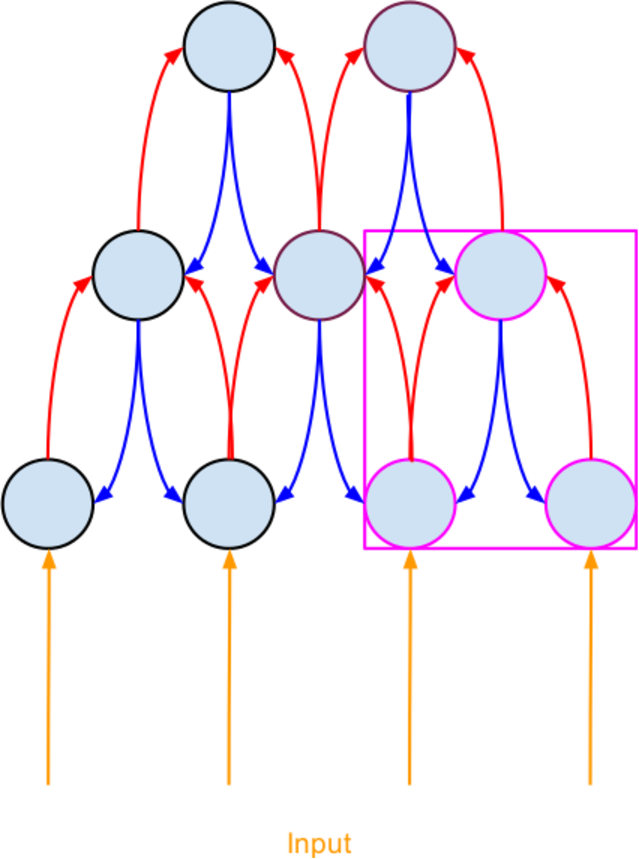
\includegraphics[width=0.5\textwidth]{pictures/perception_predictive_coding}
\end{center}
\end{figure*}

As stated above, Bayesian models account well for the results of perceptual learning experiments.
Attentional sets are crucial to the hypothesis tested in this dissertation, but they do not play a role in the conceptual and computational models of perceptual learning.
The predictive coding framework \citep{Clark2013} provides a gain-based attentional mechanism. 
In this model, attention causes greater weight to be attached to error signals from mismatched expectations and sensory input, increasing their weight and their effect on future expectations.  
However, as noted by \citet{Block2013}, this view of attention does not capture the full range of experimental results.  
For instance, in a texture segregation task, spatial attention to the periphery improves detection accuracy where spatial resolution is poor, but attention to central locations, where spatial resolution is high, actually harms accuracy \citep{Yeshurun1998}.  
This detrimental effect is an instance of missing the forest for the trees, as spatial resolution increased too much in the central locations to perceive the larger texture.  
The attentional mechanism proposed in this dissertation limits error propagation beyond where attention is focused.
Attending to perception rather than comprehension should only update expectations about perception of that individual instance.
The lower sensory levels are where stimuli are represented with the greatest degree of detail \citep{Gilbert2001}.
Perceptual learning at these lower levels should be more exposure specific and less generalized than any learning that propagates to higher representational levels.
Schema for predictive coding expectation updating under a perception-oriented attentional set and under a comprehension-oriented attentional set are shown in Figures~\ref{fig:predictivecodingperception} and~\ref{fig:predictivecodingcomprehension}, respectively.
In contrast, according to the mechanism proposed in \citet{Clark2013}, any increases in attention, perception-oriented or otherwise, are predicted to lead to greater perceptual learning.


\begin{figure*}[!ht]
\caption{A schema for predictive coding under a comprehension-oriented attentional set. Attention is represented by the green box, where it is oriented to higher, more abstract levels of sensory representation.  Error signals are able to propagate farther and update more than just the fine grained low level sensory representations. As before, blue arrows represent expectations, red arrows represent error signals, and yellow represents the sensory input.}
\label{fig:predictivecodingcomprehension}
\begin{center}
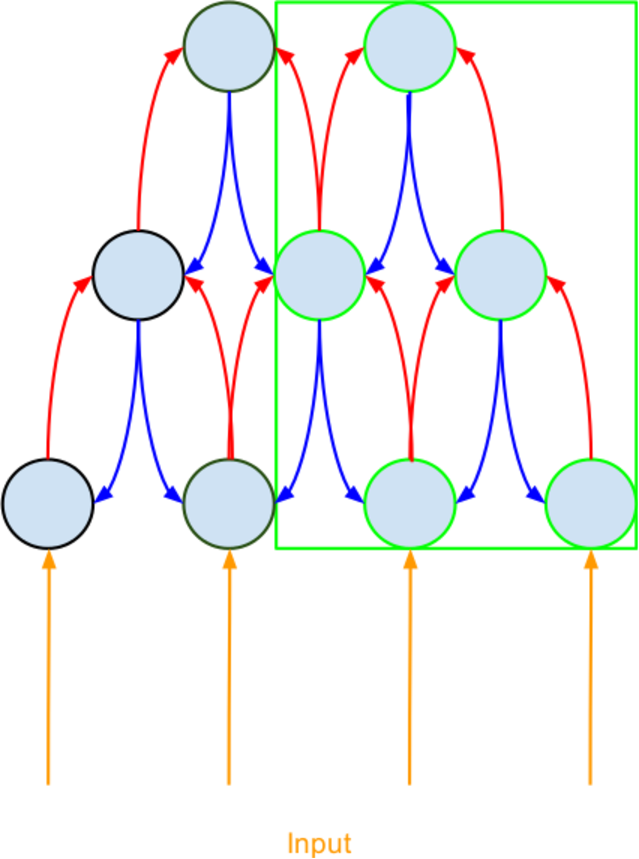
\includegraphics[width=0.5\textwidth]{pictures/comprehension_predictive_coding}
\end{center}
\end{figure*}

\section{Category typicality and perceptual learning}
\label{sec:signal}

A primary finding across the perceptual learning literature is that learning effects are found only on testing items that are similar in some sense to the exposure items.  In the most extreme instance, perceptual learning is only found on the exact same items as exposure \citep{Reinisch2014}, but most commonly, perceptual learning is limited to items produced by the same speaker as exposure \citep{Norris2003,Reinisch2013}.  However, a less studied question is what properties of the exposure items cause different degrees of perceptual learning.  

Variability is a fundamental property of the speech signal, so sound categories must have some variance associated with them and certain contexts can have increased degrees of variability.
For example, \citet{Kraljic2008a} exposed participants to ambiguous sibilants between /s/ and /\textesh/ in two different contexts.  
In one, the ambiguous sibilants were intervocalic, and in the other, they occurred as part of a /st\textturnr/ cluster in English words.  
Participants exposed to the ambiguous sound intervocalically showed a perceptual learning effect, while those exposed to the sibilants in /st\textturnr/ environments did not.  
The sibilant in /st\textturnr/ often surfaces closer to [\textesh] in many varieties of English, due to coarticulatory effects from the other consonants in the cluster.  
They argue that the interpretation of the ambiguous sound is done in context of the surrounding sounds, and only when the pronunciation variant is unexplainable from context is the variant learned and attributed to the speaker \citep[see also][]{Kraljic2008}.
In other words, a more /\textesh/-like /s/ category is typical in the context of the /st\textturnr/ clusters, but is atypical in intervocalic position.
Interestingly, given the lack of learning present in in the /st\textturnr/ context, some degree of salience seems to be required to trigger perceptual learning.

\citet{Sumner2011} investigated category typicality through a manipulation of presentation order. 
Listeners were exposed to French-accented English with modifications to the /b/-/p/ category boundary.
Participants were exposed to stimuli ranging from English-like to French-like voice onset time for /b/ and /p/.
In one presentation order, the order of stimuli was random, but in the others the voice onset time changed in a consistent manner, for instance, starting as more French-like and becoming more English-like.
The presentation order that showed the greatest perceptual learning effects was the one that began more English-like and ended more French-like.
The condition that mirrored the more normal course of nonnative speaker pronunciation changes, starting as more French-like and ending as more English-like, did not produce significantly different behavior than control participants who only completed the categorization task.
The random presentation order had perceptual learning effects in between the two ordered conditions.
These results suggest that listeners constantly update their category following each successive input, rather than only relying on initial impressions \citep[contra][]{Kraljic2008}.
This finding is mirrored in \citet{Vroomen2007}, where participants initially expand their category in response to a single, repeated modified input, but then entrench that category as subsequent input is the same.
The data in \citet{Vroomen2007} is modeled using a Bayesian framework with constant updating of beliefs.
However, in \citet{Sumner2011}, the constantly shifting condition also had more perceptual learning than a random order of the same stimuli, suggesting that small differences in expectations and observed input induce greater updating than large differences.
The bias towards small differences is better captured by the exemplar model proposed by \citet{Pierrehumbert2001}, where only input similar to the learned distribution is used for updating that distribution, and input too ambiguous given learned distributions is discarded.

Similarity of input to known distributions has effects in many psycholinguistic paradigms.
For instance in phoneme restoration, \citet{Samuel1981} found that the likelihood of restoring a sound increases when said sound is acoustically similar to the noise replacing it.  
When the replacement noise is white noise, fricatives and stops are more likely to be restored than vowels and liquids.
Simply, acoustic signals that better match expectations are less likely to be noticed as atypical.

In this dissertation, the degree of typicality of the modified category is manipulated across Experiments 1 and 2.  
In one case, the /s/ category for the speaker is maximally ambiguous between /s/ and /\textesh/, but in the other, the category is more like /\textesh/ than /s/.
The maximally ambiguous category is hypothesized to be less salient than the more /\textesh/-like /s/ category.
This lessened salience will result in greater use of comprehension-oriented attentional sets.
I hypothesize that the more /\textesh/-like category will shift listeners' attentional sets to be more perception-oriented due to their greater atypicality, which will lead to less generalized perceptual learning.  
The predictions for this hypothesis are summarized in Table~\ref{tbl:predictionsAtyp}.

\begin{table}[ht]
\caption{Summary of predictions for size of perceptual learning effects when exposed to different typicalities of the modified category.}
\label{tbl:predictionsAtyp}
\centering
\small
\begin{tabular}{cclcl}
\toprule
                     & \multicolumn{4}{c}{Lexical bias}                                                                        \\ 
\cline{2-5} 
                     & \multicolumn{2}{c}{Word-initial}                   & \multicolumn{2}{c}{Word-medial}                    \\
\cline{2-3} \cline{4-5}
 & Less atypical & More atypical  & Less atypical & More atypical  \\
\midrule
Regular attention    & Smaller effect                    & Smaller effect & Larger effect                     & Smaller effect \\
Attention to /s/     & Smaller effect                    & Smaller effect & Smaller effect                    & Smaller effect \\ \bottomrule
\end{tabular}
\end{table}

\section{Current contribution}

Lexically-guided perceptual learning generalizes to new forms and contexts far more than would be expected from a purely psychophysical perspective \citep{Norris2003,Gilbert2001}.
The two paradigms promote different attentional sets, with lexically-guided paradigms providing a focus on comprehension and psychophysics tasks giving focus to perception.  
Indeed, visually-guided perceptual learning, with its emphasis on perception of speech, shows largely similar exposure-specificity effects as the psychophysics findings \citep{Reinisch2014}.
This dissertation expands on the existing literature by modifying the exposure tasks to promote comprehension- or perception-oriented attentional sets.
Perceptual learning effects are hypothesized to be smaller in the conditions that promote perception-oriented attentional sets, as perception exposure tasks have shown greater exposure-specificity effects than comprehension exposure tasks.

